\documentclass[10pt,a4paper]{article}
\usepackage[margin=1.1cm]{geometry}
\usepackage{amsmath,amssymb}
\usepackage{graphicx}
\usepackage{booktabs}
\usepackage{caption}
\usepackage[colorlinks=true,linkcolor=blue,citecolor=blue,urlcolor=blue]{hyperref}
\usepackage[numbers,sort&compress]{natbib}
\usepackage{microtype}
\captionsetup{font=small,labelfont=bf}
\setlength{\parskip}{0pt}
\setlength{\bibsep}{1pt}
\setlength{\textfloatsep}{3pt}
\setlength{\floatsep}{4pt}
\setlength{\abovecaptionskip}{2pt}

\title{\textbf{Stall in Steady RANS Is a Branch-Selection Problem,\\ Not a Convergence Problem}}
\author{Md Mushfiqur Rahim\\
  \small ORCID: 0009-0003-1021-685X \quad Independent Researcher \\ \small AERO-BLS --- OpenFOAM v2412, NACA 0012}
\date{}

\begin{document}
\maketitle
\vspace{-2.0em}

\begin{abstract}
\noindent Two standard checks certify a steady RANS solution: grid convergence and iterative convergence. Using a 125-case campaign on the NACA 0012 (structured polar O-grids, $y^+ \approx 0.4$, $k$--$\omega$ SST with a $\gamma$--$Re_{\theta t}$ transition block), we show that at trailing-edge stall both checks pass while the answer is still wrong --- because the discrete system possesses \emph{multiple steady branches}, and neither refinement nor iteration selects among them. Under grid refinement at $\alpha = 15^\circ$ the upper-surface separation point jumps between three branches ($x/c = 0.53 \to 0.20 \to$ attached), while the same sequence is cleanly convergent at $\alpha = 5^\circ$ and $18^\circ$. A doubled-horizon URANS verification ($t^* = 0.81$--$2.4$, 61 samples) then shows the converged steady state is not an attractor: windowed means drift monotonically away from it, and at $\alpha = 15^\circ$ the steady and time-averaged drags bracket the wind-tunnel measurement. At stall, a single ``converged'' number is therefore not a well-defined object; branch envelopes and horizon-dependence must be reported instead.
\end{abstract}

\section{Introduction}
For attached flows, the certification protocol of computational aerodynamics is settled: refine the grid until a functional changes by a tolerated fraction, iterate until residuals stall, and report with a discretisation-error estimate. This letter asks what the same protocol certifies at \emph{trailing-edge stall onset}, using 125 scripted OpenFOAM runs, three-grid families at three incidences spanning the stall regime, and two time-accurate repeats with a doubled statistical horizon. The findings reduce to two statements: the steady solution set is not single-valued at stall onset (Section~\ref{sec:branches}), and the selected branch is not an attractor of the unsteady system (Section~\ref{sec:attractor}).

\section{Numerical experiment}\label{sec:setup}
Sections are meshed with Gmsh into structured polar O-grids (coarse 16{,}100, medium 33{,}740, fine 51{,}360 cells; $y^+ \approx 0.4$; farfield 20 chords, 50 for verification), closed with $k$--$\omega$ SST and, in a transition block, $\gamma$--$Re_{\theta t}$~\cite{langtry2009}. Steady cases use \texttt{simpleFoam} (4{,}000 iterations; separation from skin-friction reversal). The URANS subset uses \texttt{pimpleFoam} at $Re = 3.6\times10^5$~\cite{sheldahl1981} at $\alpha = 12^\circ$ and $15^\circ$ on the 50-chord medium grid, sampled every $0.005$~s. Baseline credibility rests on the Reynolds-matched Sandia free-transition comparison (Figure~\ref{fig:valid}): with the transition closure, pre-stall drag error falls by one third and attached-range lift is within $4$--$5\%$ of measurement; the bubble-burst stall of the experiment is not reproduced. All 125 cases, meshes, and scripts are released for end-to-end reproduction.

\begin{figure}[!htb]
  \centering
  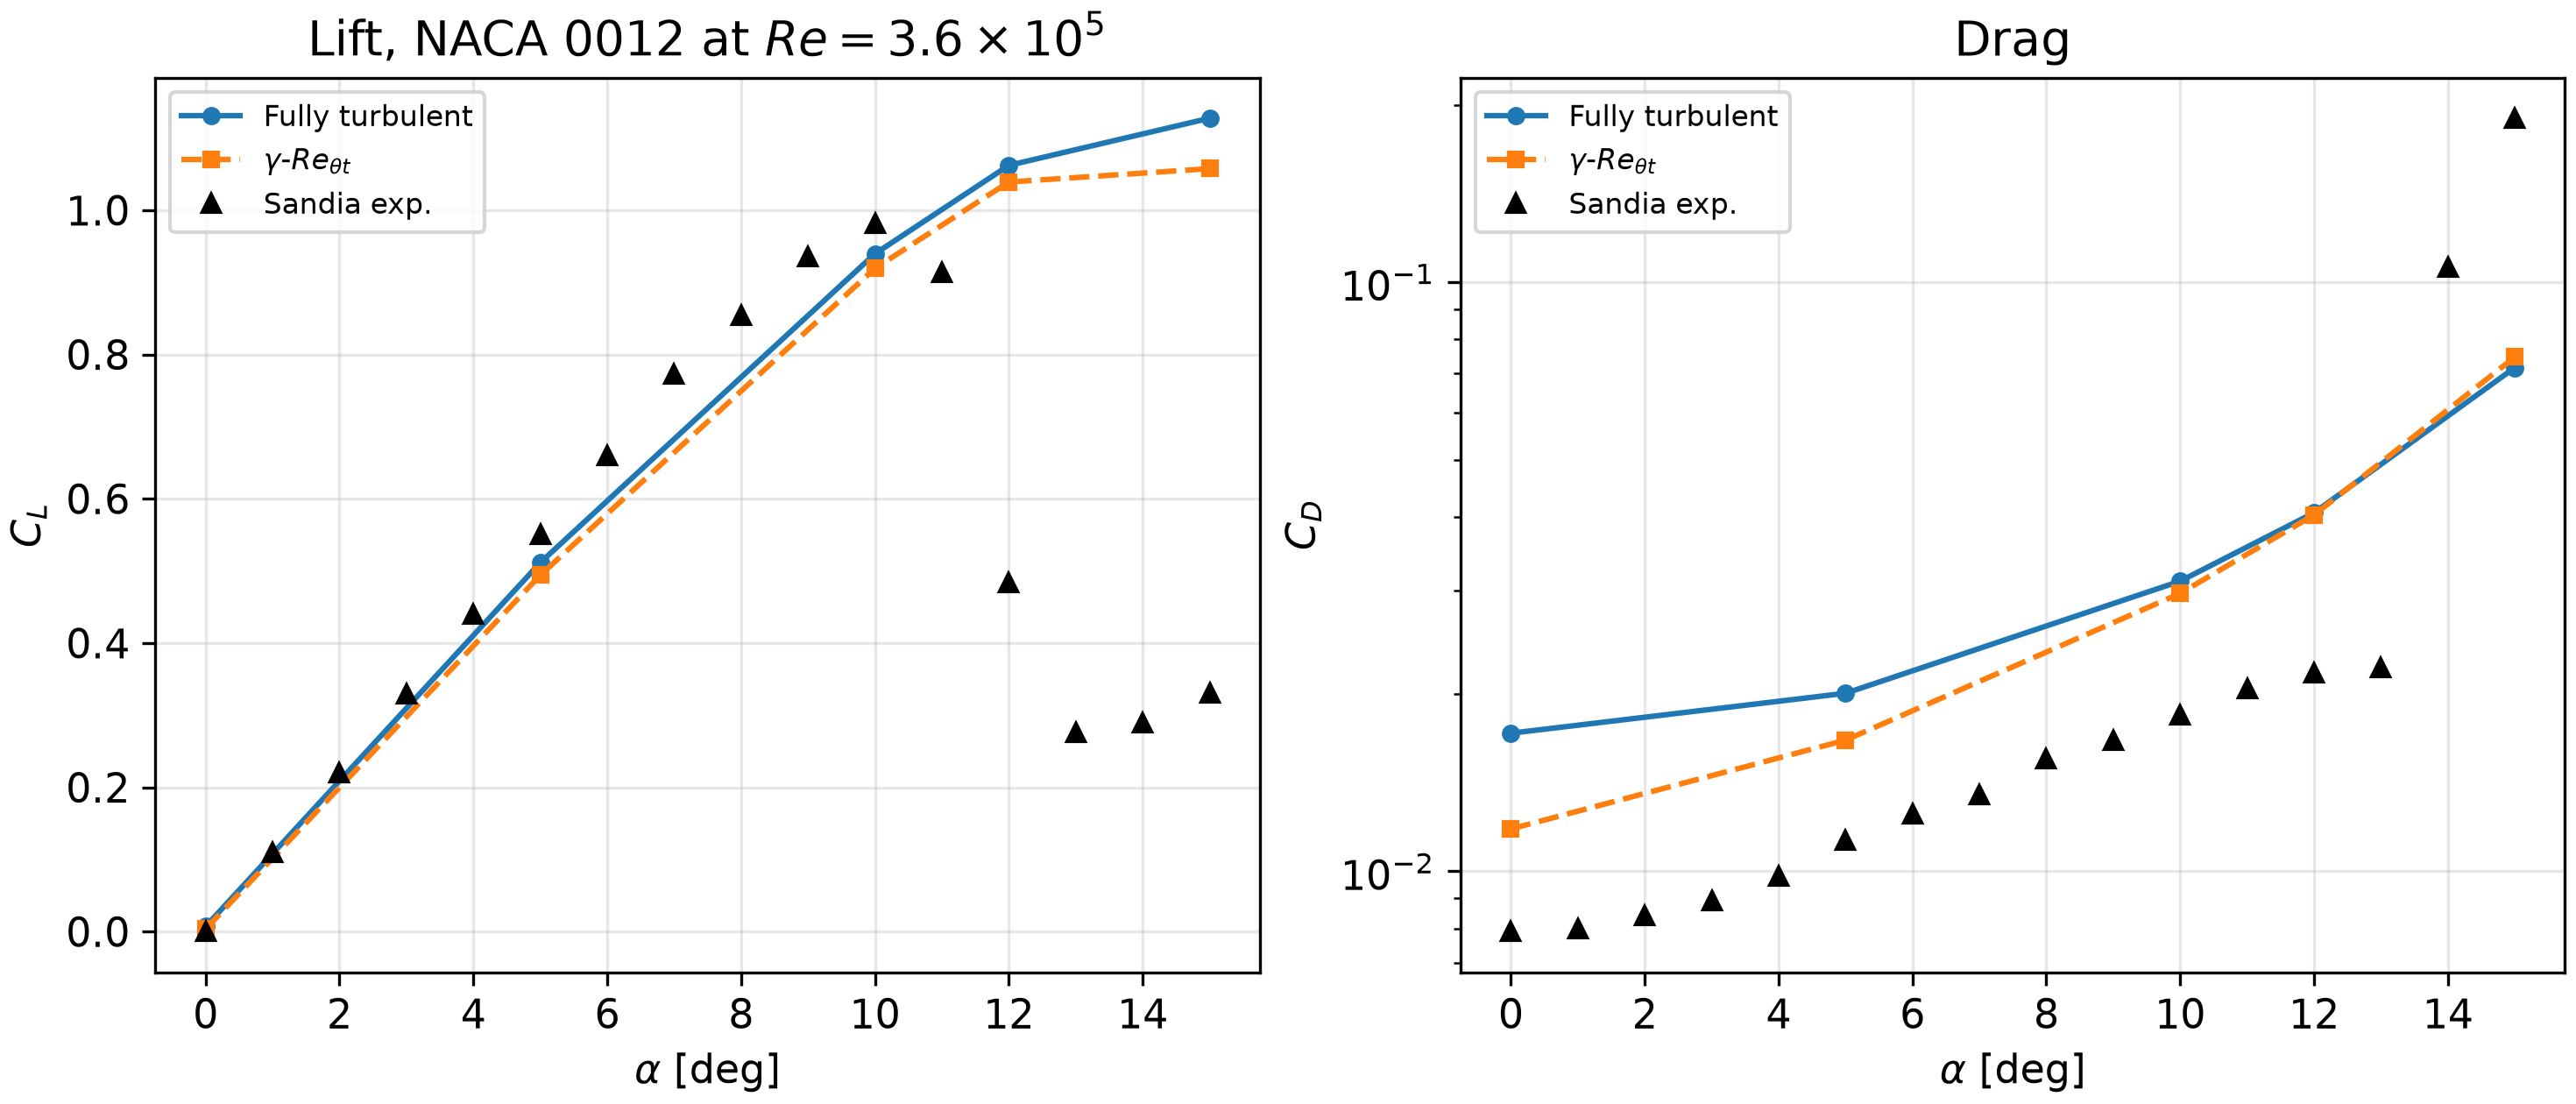
\includegraphics[width=0.28\textwidth]{figures/fig14_sandia_validation.png}
  \caption{Baseline validation: NACA 0012 at $Re = 3.6\times10^5$ with free transition against the Sandia data~\cite{sheldahl1981}.}
  \label{fig:valid}
\end{figure}

\section{Result 1: refinement does not select a branch at stall onset}\label{sec:branches}
Figure~\ref{fig:drift}a tracks the upper-surface separation point through the refinement sequence ($16{,}100 \to 33{,}740 \to 51{,}360$ cells) at three incidences; Table~\ref{tab:branch} gives the exact forces. At $\alpha = 5^\circ$ the flow is attached on every grid --- lift changes by $0.58\%$ and drag by $0.05\%$ from medium to fine. At the post-stall angle $\alpha = 18^\circ$ both grids select the \emph{same} deeply separated branch (drag within $3\%$). But at the stall-onset angle $\alpha = 15^\circ$ the three grids land on \emph{three different branches} (Table~\ref{tab:branch}) --- a $26\%$ lift spread across a monotone refinement sequence. No grid-convergence index can be formed from this family, and none should be: it is not approaching a single limit, it is hopping between basins. The medium-grid production values of the campaign are therefore a \emph{branch sample}, not a converged estimate.

\begin{table}[!htb]
  \centering\footnotesize
  \caption{Branch-map proof: the refinement family at three incidences (NACA 0012, $Re=10^6$, steady \texttt{simpleFoam}).}
  \label{tab:branch}
  \begin{tabular}{llrrrl}
    \toprule
    $\alpha$ & Grid & Cells & $C_L$ & $C_D$ & $x_{\mathrm{sep}}/c$ \\
    \midrule
    $5^\circ$  & Medium & 33{,}740 & 0.9663 & 0.0269 & attached \\
    $5^\circ$  & Fine   & 51{,}360 & 0.9724 & 0.0271 & attached \\
    $15^\circ$ & Coarse & 16{,}100 & 1.1165 & 0.0694 & 0.53 \\
    $15^\circ$ & Medium & 33{,}740 & 0.9915 & 0.0928 & 0.20 \\
    $15^\circ$ & Fine   & 51{,}360 & 1.2446 & 0.0605 & attached \\
    $18^\circ$ & Medium & 33{,}740 & 1.0175 & 0.1333 & 0.17 \\
    $18^\circ$ & Fine   & 51{,}360 & 1.1417 & 0.1292 & 0.15 \\
    \bottomrule
  \end{tabular}
\end{table}

\section{Result 2: the selected branch is not an attractor}\label{sec:attractor}
Is the selected branch at least the time-asymptotic state? The URANS repeats say no. Figure~\ref{fig:drift}b shows sliding-window means ($0.1$~s window) of the force coefficients against convective time $t^* = tU_\infty/c$ over a doubled horizon ($t^* = 0.81$--$2.4$, 61 samples; both runs required a time-step-halved restart after transition-correlation failures, with continuous histories). Three facts stand out. First, the flow is violently unsteady: the drag standard deviation is $24\%$ ($\alpha = 15^\circ$) to $41\%$ ($\alpha = 12^\circ$) of the mean. Second, the windowed means \emph{drift} --- at neither angle do they settle toward the steady branch; the mean lift excess over steady grows to $27\%$ and $34\%$ (Table~\ref{tab:uransproof}) and is still growing at the end of the window. Third, at $\alpha = 15^\circ$ the steady and extended-window URANS drags \emph{bracket} the measured value (the earlier short-horizon mean, $0.238$, sat between the two): the horizon-averaged load of this non-stationary system is a function of the averaging window, so ``the'' URANS drag is as ill-defined as ``the'' steady drag.

\begin{table}[!htb]
  \centering\footnotesize
  \caption{Non-attractor proof: steady branch vs.\ doubled-horizon URANS mean $\pm$ std ($t^* = 0.81$--$2.4$, $n = 61$) vs.\ Reynolds-matched experiment~\cite{sheldahl1981}.}
  \label{tab:uransproof}
  \begin{tabular}{lrrrrrr}
    \toprule
    & \multicolumn{3}{c}{$C_L$} & \multicolumn{3}{c}{$C_D$} \\
    \cmidrule(lr){2-4}\cmidrule(lr){5-7}
    $\alpha$ & steady & URANS & exp. & steady & URANS & exp. \\
    \midrule
    $12^\circ$ & 1.039 & $1.322 \pm 0.068$ & 0.483 & 0.040 & $0.134 \pm 0.055$ & 0.022 \\
    $15^\circ$ & 1.058 & $1.415 \pm 0.108$ & 0.331 & 0.075 & $0.307 \pm 0.073$ & 0.190 \\
    \bottomrule
  \end{tabular}
\end{table}

\begin{figure}[!htb]
  \centering
  \begin{minipage}[t]{0.44\textwidth}
    \centering
    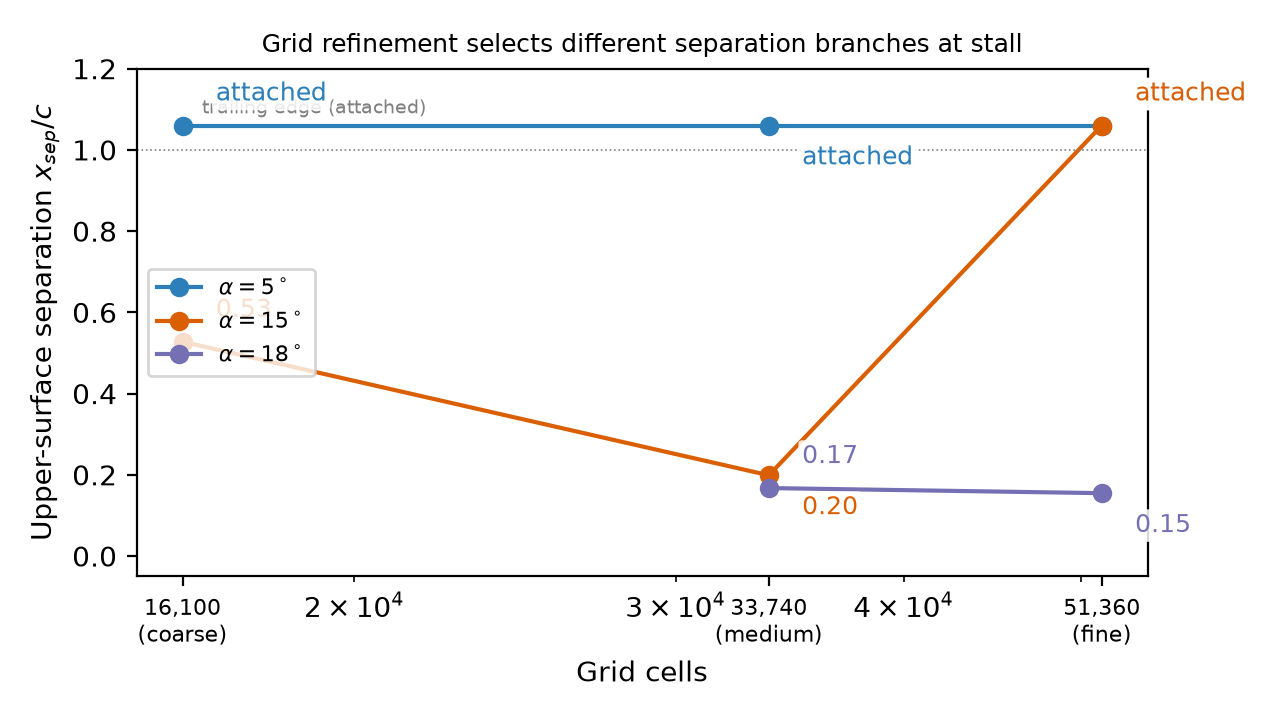
\includegraphics[width=\linewidth]{figures/figA_branch_map.png}
  \end{minipage}\hfill
  \begin{minipage}[t]{0.36\textwidth}
    \centering
    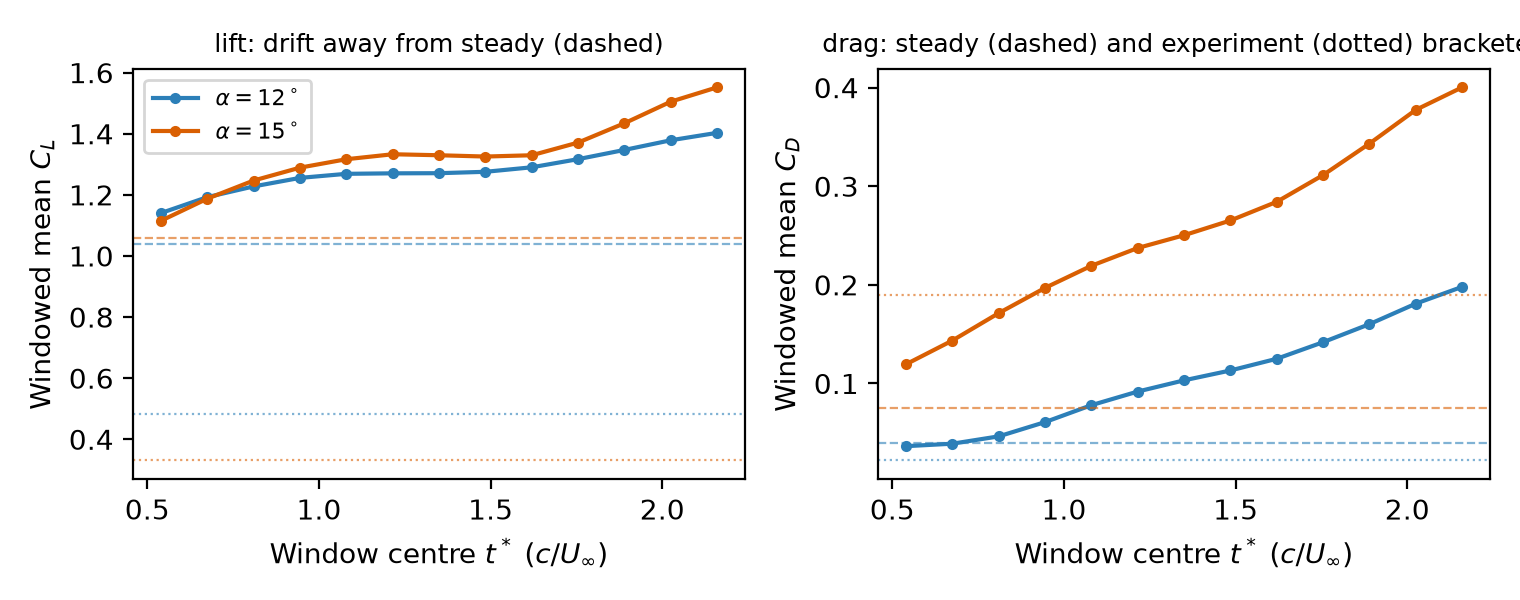
\includegraphics[width=\linewidth]{figures/figB_window_drift.png}
  \end{minipage}
  \caption{(a) Separation location through the refinement ladder: at stall onset ($\alpha = 15^\circ$) each grid selects a different branch. (b) Sliding-window means over the doubled URANS horizon (dashed: steady; dotted: experiment~\cite{sheldahl1981}); at $\alpha = 15^\circ$ (drag, right) steady and URANS bracket the measurement.}
  \label{fig:drift}
\end{figure}

\section{What follows for practice}
The failure is stall-specific, and that specificity is the useful part: attached-flow certification remains exactly as trustworthy as the protocol claims. At stall onset we suggest three reporting rules: (i) run the refinement family \emph{at the stall angle} and report the branch map --- a single-grid stall result is a draw from a discrete set, not an estimate; (ii) pair the steady solution with a time-accurate repeat, since the two can bracket the experiment from opposite sides; (iii) state the averaging horizon in convective units. None of this costs more than the standard protocol. The deeper limitation remains three-dimensional~\cite{spalart2000,mccroskey1987}: the branch structure documented here is a property of the model, not of the airfoil.

\section{Conclusion}
At trailing-edge stall onset, steady 2D RANS fails in a specific, diagnosable way: refinement hops between separation branches, iteration cannot choose among them, and the chosen branch repels the time-accurate dynamics. ``Converged'' at stall is a statement about a branch and a window, not about a number. All 125 cases, scripts, and diagnostics are openly released.

\begin{thebibliography}{9}\footnotesize
\bibitem{langtry2009} R.~B. Langtry and F.~R. Menter, \emph{AIAA Journal} 47(12):2894--2906, 2009.
\bibitem{sheldahl1981} R.~E. Sheldahl and P.~C. Klimas, Sandia Report SAND80-2114, 1981.
\bibitem{spalart2000} P.~R. Spalart, \emph{Int. J. Heat Fluid Flow} 21(3):252--263, 2000.
\bibitem{mccroskey1987} W.~J. McCroskey, NASA TM-100019, 1987.
\end{thebibliography}

\end{document}
